\documentclass{article}

\usepackage{amsmath, amsthm, amssymb, amsfonts}
\usepackage{thmtools}
\usepackage{graphicx}
\usepackage{setspace}
\usepackage{geometry}
\usepackage{float}
\usepackage{hyperref}
\usepackage[utf8]{inputenc}
\usepackage[english]{babel}
\usepackage{framed}
\usepackage[dvipsnames]{xcolor}
\usepackage{tcolorbox}
\usepackage{csquotes}
\usepackage{enumitem}
\usepackage{tikz}
\colorlet{LightGray}{White!90!Periwinkle}
\colorlet{LightOrange}{Orange!15}
\colorlet{LightGreen}{Green!15}

\newcommand{\HRule}[1]{\rule{\linewidth}{#1}}



\setstretch{1.2}
\geometry{
    textheight=9in,
    textwidth=5.5in,
    top=1in,
    headheight=12pt,
    headsep=25pt,
    footskip=30pt
}

% ------------------------------------------------------------------------------

\begin{document}

% ------------------------------------------------------------------------------
% Cover Page and ToC
% ------------------------------------------------------------------------------

\title{ \normalsize \textsc{}
		\\ [2.0cm]
		\HRule{1.5pt} \\
		\LARGE \textbf{\uppercase{Notes on Introduction to Topological Manifolds by John Lee}
		\HRule{2.0pt} \\ [0.6cm] \LARGE{} \vspace*{10\baselineskip}}
		}
\date{}
\author{\textbf{Quinten Grubbs} \\ 
		University of Missouri-St. Louis \\
		December 15 2025}

\maketitle
\newpage

\tableofcontents
\newpage

% ------------------------------------------------------------------------------

\section{Introduction}
\subsection{What are manifolds?}
\begin{itemize}
    \item Manifolds are like curves and surfaces generalized to higher dimensions.
    \item Every manifold has a dimension, which signify the number of indep. numbers needed to specify a point.
    \item An n-dimensional manifold is an object modeled locally on $\mathbb{R}^n$.
    \item 1-dimensional manifolds are commonly called "curves" (1 coordinate is needed to specify a value on the curve)
    \item 2-dimensional manifolds are "surfaces, most common examples are planes and spheres. (2-coordinates are needed to specify a point on the surface)
    \item An n-dimensional manifold "looks like" $\mathbb{R}^n$ locally.
\end{itemize}
Now we must begin constructing definitions to formalize this notion of being locally "like" $\mathbb{R}^n$.\\
We say that two subsets of Euclidean spaces $U\subset \mathbb{R}^k$, $V\subset\mathbb{R}^n$ are topologically equivalent or homeomorphic if there exists a one-to-one correspondence $\phi: U\to V$ such that both $\phi$ and its inverse are continuous maps.\\
We also say a subset $M$ of some Euclidean space $\mathbb{R}^k$ is locally euclidean of dimension $n$ if every point of $M$ has a neighborhood in $M$ that is topologically equivalent to a ball in $\mathbb{R}^n$.\\
This gives us a preliminary definition of a manifold.\\
\textbf{Def: } An $n$-dimensional manifold is a subset of some Euclidean space $\mathbb{R}^k$ that is locally Euclidean of some dimension $n$.

\section{Topological Spaces}
\begin{itemize}
    \item A problem with the prior definition of manifolds is that it depends on having "an ambient Euclidean space" in which the manifold lives.
\end{itemize}
A topology on a set $X$ is a collection $\mathcal{T}$ of subsets of $X$, called open sets, such that:
\begin{enumerate}
    \item $X$ and $\emptyset$ are elements of $\mathcal{T}$.
    \item $\mathcal{T}$ is closed under finite intersections: If $U_1,...,U_n\in \mathcal{T}$, then their intersection $U_1\cap...\cap U_n$ is in $\mathcal{T}$
    \item $\mathcal{T}$ is closed under arbitrary unions: If $\{U_\alpha\}_{\alpha\in A}$ is any (finite or infinite) collection of elements of $\mathcal{T}$, then their union $\bigcup_{\alpha\in A}U_\alpha$ is in $\mathcal{T}$.
 \end{enumerate}
 \begin{itemize}
     \item If $X$ is a topological space and $q\in X$, a neighborhood of $q$ is an open set containing $q$.
 \end{itemize}
 \subsection{Convergence and Continuity}
 Topological spaces provide the most general setting for studying the notions of convergence and continuity.\\
 \textbf{Definition of Convergence:} If $X$ is a topological space and $\{q_i\}$ is any sequence of points in $X$, we say that the sequence \textit{converges} to $q\in X$ and is the limit of the sequence, if for every neighborhood $U$ of $q$ there exists $N$ such that $q_i\in U$ for all $i\geq N$.\\
 \\
 \textbf{Exercise 2.3(a): }Let $X$ be a discrete topological space. Show that the only convergent sequences in $X$ are the ones that are "eventually constant," that is, sequences $\{q_i\}$ such that $q_i=q$ for all $i$ greater than some $N$.\\
 \\
 \textbf{Proof: } Assume that $\{q_i\}$ is a convergent sequence to $q$ in $X$. Then it follows that for every neighborhood $U$ of $q\in X$ there exists $N$ such that $q_i\in U$ for all $i\geq N$. Now let the neighborhood of $q$ be $U=\{q\}$. Then it follows that there exists $N$ such that $q_i\in U$ for all $i\geq N$. Thus, the sequence must eventually become constant to the value $q$. $\square$.\\
 \\
 Now we look at continous maps and their topological definition.\\
 \textbf{Continuous Function:} If $X$ and $Y$ are topological spaces, a map $f:X\to Y$ is said to be continuous if for every open set $U\subset Y$, $f^{-1}(U)$ is open in $X$.\\
 \\
 We now give some elementary properties of continuous functions.\\

 \textbf{Lemma 2.1:} Let $X,Y,Z$ be topological spaces\\
 \begin{enumerate}
     \item Any constant map $f:X\to Y$ is continuous.
     \item The identity map $Id: X\to X$ is continuous.
     \item If $f:X\to Y$ is continuous, so is the restriction of $f$ to any open subset.
     \item If $f:X\to Y$ and $g:Y\to Z$ are continuous, so is their composition $g\circ f:X\to Z$.
 \end{enumerate}
\vspace{\baselineskip}
\textbf{Exercise 2.4: Prove parts a-c.}\\
\textbf{Proof (a):} Let $f:X\to Y$ be the constant map where $f(x) = a$ for all $x\in X$ and some $y\in Y$. Let $U$ be an open set in $Y$. Then it follows that $f^{-1}(U)=X$ if $y\in U$ and $f^{-1}(U) = \emptyset$ if $y\notin U$. Thus the inverse image of any open set in $Y$ is always open.$\square$.\\
\textbf{Proof (b):} Let $f:X\to X$ be the identity map. Now let $U$ be an open set in $X$. Then it follows that $f^{-1}(U)=U$ and the inverse of an open set is the open set itself.$\square$.\\
\textbf{Proof (c):} Assume that $f:X\to Y$ is continuous. Then it follows that for every open set $U\in Y$ that $Z=f^{-1}(U)$ is open. Now take the restriction of $f$ to some open set $V\in X$. Then it follows that $f^{-1}_V(U) = Z \cap V$. We know that topologies include the intersection of two open sets. Thus, $Z\cap V$ is open. $\square.$\\

Now we want to look at the definition for local continuity of a function.\\
\\
\textbf{Local Criterion for Continuity:} A map $f:X\to Y$ between topological spaces is continuous if and only if each point of $X$ has a neighborhood on which $f$ is continuous.

\begin{itemize}
    \item If $X$ and $Y$ are topological spaces, a homeomorphism from $X$ to $Y$ is defined to be a continuous bijective map $\phi:X\to Y$ with continuous inverse.
    \item If there exists a homeomorphism between $X$ and $Y$ we say that $X$ and $Y$ are homeomorphic denoted $X\approx Y$.
\end{itemize}
\textbf{Exercise 2.5: show that homeomorphic is an equivalence relation.}\\
\textbf{Work:}
\begin{itemize}
    \item \textbf{Reflexitivity:} $X$ is homeomorphic to itself from the identity map.
    \item \textbf{Symmetry} Assume WLG that $X\approx Y$. Then it follows that there exists continous $f:X\to Y$ such that $f^{-1}$ is continuous. For $Y\approx X$, we simply take $f^{-1}$ as our homeomorphism.
    \item \textbf{Transitivity:} If we assume $X\approx Y$ and $Y\approx Z$, then there exists homeomorphisms $f:X\to Y$ and $g:Y\to Z$. Take the function $g\circ f:X\to Z$. We know this composition is continuous and its inverse is as well. Thus, $X\approx Z$.
\end{itemize}
A map $f:X\to Y$ is said to be an open map if for any open set $U\subset X$, the image $f(U)$ is open in $Y$.\\
We can also construct a useful generalization of homeomorphisms.\\
\textbf{Local Homeomorphism:} We say a continuous map $f:X\to Y$ is a local homeomorphism if every point $x\in X$ has a neighborhood $U\subset X$ such that $f(U)$ is an open subset of $Y$ and $f|_U:U\to f(U)$ is a homeomorphism.\\
\\
\textbf{Exercise 2.8: }
\begin{enumerate}
    \item Show that every local homeomorphism is an open map.
    \item  Show that every homeomorphism is a local homeomorphism.
    \item Show that a bijective continuous open map is a homeomorphism.
    \item Show that a bijective local homeomorphism is a homeomorphism.
\end{enumerate}
\textbf{Proof (1):} Assume that $f:X\to Y$ is a local homeomorphism. Let $U\subset X$ be an open set in $X$. We know that every point $x\in X$ has a neighborhood $V$ such that $f(V)$ is open. Take an arbitrary collection of these neighborhoods $\bigcup\limits_\alpha V_\alpha$ until $U\subset \bigcup\limits_\alpha V_\alpha$. It follows then that each restriction of $f$, $f|_{V_\alpha}$ is a homeomorphism. Thus, for every open set $O$ in $V_\alpha$ it follows that $f(O)$ is open. Since, $U\subset \bigcup\limits_{\alpha} V_\alpha$ we can construct $U=\bigcup\limits_{\alpha}O_\alpha$ where each $O_\alpha=U\cap V_\alpha$. Thus, $f(U)=f(\bigcup\limits_\alpha O_\alpha)=\bigcup\limits_\alpha f(O_\alpha)$. Therefore, $f(U)$ is the union of open sets and is open itself. $\square$.\\
\\
\textbf{Proof (2):} Assume that $f:X\to Y$ is a homeomorphism. Since $f^{-1}$ is continuous (by the definition of a homeomorphism) every open set $U\subset X$ implies that $f(U)$ is open. $\square$.\\
\\
\textbf{Proof (3):} Assume that $f:X\to Y$ is bijective continuous open map. Since $f$ is bijective, we know that $f^{-1}$ exists. We also know that for every open set, $U\subset X$ that $f(U)$ is open. Therefore, $f^{-1}$ is continuous. We have that $f$ is continuous by our assumption. Thus, $f$ is a homeomorphism. $\square$.\\
\\
\textbf{Proof (4):} Assume that $f:X\to Y$ is a bijective local homeomorphism.

\subsection{Closed Sets}
A subset $F$ of a space $X$, is said to be \textbf{closed} if its complement $X\setminus F$ is open. Closed sets have the following properties:
\begin{enumerate}
    \item $X$ and $\emptyset$ are closed.
    \item Finite unions of closed sets are closed.
    \item Arbitrary intersection of closed sets are closed.
\end{enumerate}
We can also redefine continuity in terms of open sets:\\
\textbf{Lemma 2.7:} A map between topological spaces is continuous if and only if the inverse image of every closed set is closed.\\
\\
\textbf{Exercise 2.9: Prove this Lemma}\\
\textbf{Proof:} $(\to)$ Assume $f:X\to Y$ is continuous. Then if $U$ is an open set in $Y$ implies that $f^{-1}(U)$ is open in $X$. Therefore, by definition for any closed set $Y\setminus U$, it follows that $X\setminus f^{-1}(U)$ is closed. It follows from set-theory that $f^{-1}(Y\setminus U)=X\setminus f^{-1}(U)$.\\
\\
$(\leftarrow)$ Assume that the inverse image of every closed set is closed. Then for every closed set $U$ in $Y$ it follows that $f^{-1}(U)$ is closed. Then it follows that $Y\setminus U$ is open and $X\setminus f^{-1}(U)=f^{-1}(Y\setminus U)$ is open. $\square$.\\
\\
We define two sets:
\begin{itemize}
    \item The "Closure of $A$",\\
    $\bar{A}=\bigcap\{B\subset X: B\supset A \text{ and } B \text{ is closed in $X$}\}$.
    \item The "Interior of $A$",\\
    $Int A=\bigcup\{C\subset X: C \subset A \text{ and $C$ is open in $X$}\}$.
    \item We define the "exterior of A",\\
    $ExtA=X\setminus\bar{A}$.
    \item We define the "boundary of $A$",\\
    $\partial A=X\setminus (IntA\cup ExtA)$.
\end{itemize}

These definitions now lead us to the following lemma:\\
\textbf{Lemma 2.8:} Let $X$ be a topological space and $A\subset X$ any subset.
\begin{enumerate}[label=(\alph*.)]
    \item A point q is in the interior of A if and only if q has a neighborhood contained in A.
    \item A point q is in the exterior of A if and only if q has a neighborhood contained in $X\setminus A$.
    \item A point q is in the boundary of A if and only if every neighborhood of q contains both a point of A and a point of $X\setminus A$.
    \item $Int A$ and $Ext A$ are open in $X$, while $\partial A$ is closed in $X$
    \item A is open if and only if $A=Int A$
    \item $A$ is closed iff it contains all its boundary points, which is true iff $A=IntA\cup \partial A$.
    \item $\bar{A}=A\cup\partial A=IntA\cup\partial A$
\end{enumerate}
\vspace{\baselineskip}
\textbf{Exercise 2.10: Prove Lemma 2.8}\\
I will not prove all of these as some of them are ridiculously trivial, but I will select those that seem somewhat nontrivial.\\
\textbf{Proof (a.):} By definition.\\
\textbf{Proof (b.):} By definition.\\
\textbf{Proof (c.):} Here, we use the previous facts with their negations. Therefore,
\begin{itemize}
    \item A point q is not in the interior if and only if every neighborhood of q is not contained in $A$.
    \item A point q is not in the exterior of $A$ if and only if every neighborhood of $q$ is not contained in $X\setminus A$.
\end{itemize}
$(\to)$Now, assume $q$ is in the boundary of $A$. Then, $q\notin IntA$ and $q\notin ExtA$. Therefore, by (1) every neighborhood is not contained A and has a point in $X\setminus A$. By (2) every neighborhood is not contained in $X\setminus A$ and thus has a point in $A$. The other direction is almost exactly the same. $\square$.\\
\textbf{Proof (d.):} These are trivial.\\
\textbf{proof (e.):} Skipped\\
\textbf{Proof (f.):} We first prove the first statement.\\
$(\to)$ Assume that $A$ is closed. It follows that $A=\bar{A}$ since $\bar{A}$ is the smallest closed set which contains $A$ and $A$ is closed. We can write $X=IntA\sqcup \partial A \sqcup Ext A$. Since $A=\bar{A}$, it follows that $ExtA=X\setminus A$. Therefore, $X=Int A\sqcup \partial A \sqcup (X\setminus A)$. Thus, $A=IntA\sqcup \partial A$ and $A$ contains all its boundary points.\\
$(\leftarrow)$ Assume that $\partial A\subset A$. Then it follows that $A=Int(A)\sqcup \partial A$. Taking $X=Int(A)\sqcup\partial A\sqcup Ext(A)$, we see that $A$ is the complement of an open set $Ext(A)$. Thus, $A$ is closed. $\square$.
\\
\textbf{Proof (g.):} Uses same logic as before.\\

Given a top. space $X$ and a set $A\subset X$, we say that a point $q\in X$ is a limit point of $A$ if every neighborhood of $q$ contains a point of $A$ other than $q$.\\
\\
\textbf{Exercise 2.11:} Show that a set $A$ in top. space is closed iff it contains all its limit points.\\
\textbf{Proof:}\\
$(\to)$ Assume that $A$ is closed. Then it follows that $X\setminus A$ is open. Therefore, for every $p\in X\setminus A$ there is an open neighborhood $p\in U\subset X\setminus A$ entirely contained in $X\setminus A$. Therefore, $p$ is not a limit point of $A$. Thus, all limit points of $A$ must be in $A$.\\
$(\leftarrow)$ Assume that $A$ contains all its limit points. By definition we know that $IntA\subset A$. Now let $x\in \partial A$. Then it follows that every neighborhood of $x$ contains a point in $A$ and a point in $X\setminus A$. Assume for a contradiction that $x\in X\setminus A$. Then every neighborhood of $x$ contains a point of $A$ other than $x$. Thus, $x$ is a limit point of $A$ and must be in $A$, a contradiction. Therefore, $x\in A$. This means $\partial A\subset A$ and $A=\bar{A}$. $\square$.\\

\subsection{Bases}
\textbf{Definition of Basis:} Suppose $X$ is any set. A basis in $X$ is a collection $\mathcal{B}$ of subsets of $X$ satisfying:
\begin{enumerate}
    \item Every element of $X$ is in some element of $\mathcal{B}$; in other words,
    $X=\bigcup_{B\in\mathcal{B}}B$.
    \item If $B_1,B_2\in \mathcal{B}$ and $x\in B_1\cap B_2$, there exists an element $B_3\in \mathcal{B}$ such that $x\in B_3\subset B_1\cap B_2$.
\end{enumerate}
Using this definition we can build a topology:\\
\textbf{Proposition 2.9:} Let $\mathcal{B}$ be a basis in a set $X$, and let $\mathcal{T}$ be the collection of all unions of elements of $\mathcal{B}$. Then $\mathcal{T}$ is a topology on $X$.\\
\textbf{Basis Criterion:} Given $X$ and a collection $\mathcal{B}$ of subsets of $X$, we say that a subset $U\subset X$ satisfies the basis criterion with respect to $\mathcal{B}$ if for every $x\in U$, there exists $B\in\mathcal{B}$ such that $x\in B \subset U$.

\textbf{Lemma 2.10: } Suppose $\mathcal{B}$ is a basis in $X$. Then the collection $\mathcal{T}$ defined in prop 2.9 is precisely the set of all subsets of $X$ that satisfy the basis criterion with respect to $\mathcal{B}$.\\

\textbf{Proof of Lemma 2.10: }\\
Let $U\subset X$, and suppose that $U$ satisfies the basis criterion.\\
Let $V=\bigcup\{B\in\mathcal{B}:B\subset U\}$. Since $V$ is a union of basis sets, $V\in \mathcal{T}$. If we show that $U=V$, it will follow that $U\in \mathcal{T}$. Clearly $V\subset U$ as every subset that forms $V$ is a subset of $U$. Now we wish to show that $U\subset V$. Let $x\in U$. Since $U$ satisfies that Basis criterion, the must exist basis set $B\in\mathcal{B}$ such that $x\in B\subset U$. Therefore, $x\in V$.\\
Conversely, suppose that $U\in \mathcal {T}$. Thus $U$ is a union of elements of $\mathcal{B}$, i.e. for some $A\subset \mathcal{B}$, $U=\bigcup_{B\in A} B$. In other words, $x\in U$ iff $x\in B$ for some $B\in A$.In particular, $x\in B\subset U$, so $U$ satisfies the basis criterion. $\square$.\\
\\
The following lemma can provide an easier way to show that a topology $\mathcal{T}$ can be generated by some basis $\mathcal{B}$.\\
\textbf{Lemma 2.11:} Suppose $X$ is a topological space, and $\mathcal{B}$ is a collection of open subsets of $X$. If every open subset of $X$ satisfies the basis criterion with respect to $\mathcal{B}$, then $\mathcal{B}$ is a basis for the topology of $X$.\\
\\
\textbf{Exercise 2.15:} In each of the following cases, prove that the given set $\mathcal{B}$ is a basis for the given topology.\\
\begin{enumerate}[label=(\alph*.)]
    \item  $X$ is a set with the discrete topology, and $\mathcal{B}$ is the collection of all
    one-point subsets of $X$.
    \item X is a set with the trivial topology, and $\mathcal{B} = \{X\}$.
\end{enumerate}
\textbf{Proof (a.):} Assume $X$ is a set with the discrete topology $\mathcal{T}$, and $\mathcal{B}$ is the collection of all one-point subsets of $X$. Now let $x\in U$ where $U\in \mathcal{T}$. We know that there exists $B\in\mathcal{B}$ so that $x\in B$ as it contains a set containing each point in $X$. It is obvious that $B\subset U$, since $B$ contains only $x$ and $U$ contains $x$ and potentially other elements. Therefore, every set $U\in \mathcal{T}$ satisfies the basis criterion. $\square$.\\
\\
\textbf{Proof (b.):} Assume $X$ is a set with the trivial topology, and $\mathcal{B}=\{X\}$. We simply just need to show that $\emptyset, X$ satisfy the basis criterion. For the open set $\emptyset$. There are no points in $\emptyset$ so it vacuosly satisfies the basis criterion. Now, the other open set $X$. Let $x\in X$. Then it follows that $x\in X\subset X$. $\square$.\\
\\
Checking basis sets gives us a much easier way to define continuity.\\
\textbf{Lemma 2.12:} Let $X$ and $Y$ be topological spaces and let $\mathcal{B}$ be a basis for $Y$. A map $f:X\to Y$ is continuous if and only if for every basis open set $B\in \mathcal{B}$, $f^{-1}(B)$ is open in $X$.\\
\subsection{Manifolds}
Let $X$ be a topological space. A topological space $M$ is said to be locally Euclidean of dimension $n$ if every point $q\in M$ has a neighborhood that is homeomorphic to an open subset of $\mathbb{R}^n$. Such a neighborhood is called a Euclidean neighborhood of $q$. The following lemma specifies how we usually characterize locally Euclidean spaces.\\
\textbf{Lemma 2.12:} A topological space $M$ is locally Euclidean of dimension $n$ iff either of the following properties holds:
\begin{enumerate}[label=[(\alph*.)]
    \item Every point of $M$ has a neighborhood homeomorphic to an open ball in $\mathbb{R}^n$.
    \item Every point of $M$ has a neighborhood homeomorphic to $\mathbb{R}^n$
\end{enumerate}
\begin{itemize}
    \item If $M$ is locally Euclidean of dimension $n$, a homeomorphism from an open subset $U\subset M$ to an open subset of $\mathbb{R}^n$ is called a \textbf{coordinate chart} on $U$.
    \item We will call any open subset of $M$ that is homeomorphic to a ball in $\mathbb{R}^n$ a \textbf{Euclidean ball} in $M$.
\end{itemize}
\subsection{Hausdorff Spaces}
We introduce a property to ensure that there are enough open sets, so that neighborhoods behave more or less how our intuition expects.
\begin{itemize}
    \item A topological space $X$ is said to be a \textbf{Hausdorff space} if given any pair of distinct points $q_1,q_2\in X$, there exist neighborhoods $U_1$ of $q_1$ and $U_2$ of $q_2$ with $U_1\cap U_2=\emptyset$.
    \item Any metric space if Hausdorff.
    \item Any open subset of a Hausdorff space is Hausdorff.
\end{itemize}
Hausdorff have many properties reminiscent of metric spaces.\\
\textbf{Lemma 2.14:} Let $X$ be a Hausdorff Space.
\begin{enumerate}[label=(\alph*.)]
    \item Every one-point set in $X$ is closed.
    \item If a sequence $\{x_i\}$ in $X$ converges to a limit $x\in X$, the limit is unique.
\end{enumerate}
Now let's prove both of these properties:\\
\textbf{Proof (a.):} Assume $X$ is a Hausdorff space. Now let $q_0\in X$. Let $p\in X$ be the point for our one-point set $A=\{p\}$. Assume $p\neq q$. Then it follows that there exist neighborhoods $U_p,U_q$ s.t. $U_p\cap U_q=\emptyset$. Since $q_0$ is an arbitrary point not in $A$, it follows that we can write $X\setminus A$ as a union of these open sets containing $q_0$. Therefore, $X\setminus A$ is open. $\square$.\\
\textbf{Proof (b.):} Assume that $X$ is a Hausdorff space. Assume that a sequence converges to a limit $x\in X$ and $y\in X$. Then for every neighborhood $U_x$ of $x$ and $U_y$ of $y$, there exists $N_x$ and $N_y$ such that $x_i\in U_x$ for all $i\geq N_x$ and $x_i\in U_y$ for all $i\geq N_y$. Now take $i\geq max(N_x, N_y)$. Then $x_i\in U_x$ and $x_i \in U_y$. Take these neighborhoods to be Hausdorff. Then there is a contradiction. $\square$\\
\textbf{Exercise 2.17:} Show that the only Hausdorff topology on a finite set is the discrete topology.\\
\textbf{Proof:} Assume $\mathcal{T}$ is a Hausdorff topology on a finite set $X$. Then it follows that for two points $p,q\in X$ each has a neighborhood $U_p,U_q\in\mathcal{T}$ s.t. $U_p\cap U_q=\emptyset$. Let $q$ be an arbitrary point in $X$. Then it follows that each pair $(p,q)$ have neighborhoods $(U_p,U_q)$ with no overlap for every $q\in X$. Taking the intersection of each $U_p$ generated from its pairing with $U_q$ we see that it must be the set $\{p\}$. Therefore, $\mathcal{T}$ contains every set which consists of a single point in $X$. This generates the discrete topology on $X$. $\square$.
\subsection{Second Countability}
We say that a topological space is \textbf{second countable} if it admits a countable basis.\\
(This ensures that there are not too many open sets for our manifold.)\\
There is also weaker notion of second countability which we will need another definition to state:\\
\textbf{Definition:} If $X$ is a space and $q\in X$, a collection $\mathcal{B}_q$ of neighborhoods of $q$ is called a \textbf{neighborhood basis} at $q$ if every neighborhood of $q$ contains some $B\in\mathcal{B}_q$.\\
\\
\textbf{Definition:} $X$ is said to be \textbf{first countable} if there exists a countable neighborhood basis at each point.
\begin{itemize}
    \item Second countability implies first countability.
    \item If $X$ is any topological space, a collection $\mathcal{U}$ of subsets of $X$ is said to \textit{cover} $X$, or to be a cover of $X$, if every point in $X$ is in one of the sets of $\mathcal{U}$.
    \item An \textit{open cover} of $X$ is a collection of open sets that covers $X$.
    \item Given any cover $\mathcal{U}$, a \textit{subcover} of $\mathcal{U}$ is a subset of $\mathcal{U}$ that is still a cover.
\end{itemize}
\textbf{Lemma 2.15:} If $X$ is a second countable space, every open cover of $X$ has a countable subcover.\\
Let's look at the proof to gather a better intuition of second countability.\\
\textbf{Proof:} Let $\mathcal{B}$ be a countable basis for $X$, and let $\mathcal{U}$ be an arbitrary open cover of $X$. let $\mathcal{B}'$ denote the subset of $\mathcal{B}$ consisting of these basis sets that are entirely contained in some element of $\mathcal{U}$. Because any subset of a countable subset is countable, $\mathcal{B}'$ is a countable set.\\
Now, for each element $B\in\mathcal{B}'$, choose an element $U_B\in \mathcal{U}$ such that $B\subset U_B$. The collection $\mathcal{U}'=\{U_B:B\in\mathcal{B}'\}$ is a countable subset of $\mathcal{U}$; We just need to show that $\mathcal{U}'$ still covers $X$.\\
If $x\in X$ is arbitrary, then $x\in U_0$ for some open set $U_0\in\mathcal{U}$. By the basis criterion for $U_0$, there is some $B\in\mathcal{B}$ such that $x\in B\subset U_0$. This means, that $B\in \mathcal{B}'$ and therefore there is a set $U_B\in \mathcal{U}'$ such that $x\in B\subset U_B$. $\square$.
\begin{itemize}
    \item Most reasonable spaces are second countable.
    \item Any open subset $U$ of a second countable space $X$ is second countable.
\end{itemize}
\subsection{Definition of Manifolds}
We have now defined enough to give the formal definition of a manifold:\\
\\
\textbf{Definition of Manifold:} An $n$-dimensional topological manifold is a second countable Hausdorff space that is locally Euclidean of dimension $n$.\\
(This text will not discuss other types of manifolds such as "smooth manifolds" or "complex manifolds".)
\begin{itemize}
    \item We define a shorthand $M^n$ is a shorthand for $M$ is a manifold of dimension $n$.
    \item The most obvious example of an $n$-manifold is $\mathbb{R}^n$ itself.
\end{itemize}
\textbf{Lemma 2.16:} Any open subset of an $n$-manifold is an $n$-manifold.\\
\\
\textbf{Proof:} Let $M$ be an $n$-manifold, and let $V$ be an open subset of $M$. We know from previous lemmas that $V$ must also be Hausdorff and second countable. Thus, we just need to show that $V$ is locally Euclidean. Any $q\in V$ has a neighborhood (in M) that is homeomorphic to an open subset of $\mathbb{R}^n$; Taking the intersection of that neighborhood with $V$, gives us an open set homeomorphic to an open subset of $\mathbb{R}^n$ contained in $V$. Thus, V is locally Euclidean. $\square$.\\

\subsection{Manifolds with Boundary}
We can also construct a more general notion.
\begin{itemize}
    \item An $n$-dimensional manifold with boundary is a second countable Hausdorff space in which every point has a neighborhood homeomorphic to an open subset of the $n$-dimensional upper half space $\mathbb{H}^n=\{(x_1,...,x_n)\in\mathbb{R}^n:x_n\geq 0\}$.
    \item we call any homeomorphism for an open subset $U\subset M$ to an open subset of $\mathbb{H}^n$ a chart on $U$.
    \item The boundary of $\mathbb{H}^n$ in $\mathbb{R}^n$ is the set of points where $x_n=0$.
    \item If $M$ is a manifold with boundary, a point that is in the inverse image of $\partial\mathbb{H}^n$ under some chart is called a boundary point of $M$.
    \item A point that is in the inverse image of $Int\mathbb{H}^n$ is called an interior point.
    \item The boundary of $M$ is denoted by $\partial M$, its interior is denoted $Int M$. These are distinct from the earlier definitions of Int and $\partial$.
\end{itemize}
\subsection{Problems}
\textbf{Problem 1:} Let $(X_1, \mathcal{T}_1)$ and $(X_2,\mathcal{T})$ be topological spaces and let $f:X_1\to X_2$ be a bijective map. Show that $f$ is a homeomorphism if and only if $f(\mathcal{T}_1)=\mathcal{T}_2$ in the sense that $U\in\mathcal{T}_1$ iff $f(U)\in \mathcal{T}_2$.\\
\\
\textbf{Proof:} $(\to)$ Assume $f$ is a homeomorphism. Since $f^{-1}$ is continuous, it follows that for all $U\in\mathcal{T}_1$ that $f(U)\in \mathcal{T}_2$. Now let $f(U)\in\mathcal{T}$. Then since $f$ is continuous, it follows that $f^{-1}f(U)$ is open. Thus, $U\in \mathcal{T}_1$.\\
\\
$(\leftarrow)$ Assume $f(\mathcal{T}_1 ) = \mathcal{T}_2$. Then it follows that if $U$ is open in $X$, then $f(U)\in\mathcal{T}_2$. Thus, $f^{-1}$ is continuous. We also know that since $f$ is surjective every open set $V\in \mathcal{T}_2$ can be written as $f(Z)$, where $Z\subset X$. By our assumption, since $V=f(Z)$ is open this means that $Z\in\mathcal{T}_1$. $\square$.
\section{New Spaces from Old}
New and interesting ways to generate spaces are given in this chapter.
\subsection{Subspaces}
\begin{itemize}
    \item Let $X$ be a space, and let $A\subset X$ be any subset. We define a topology $\mathcal{T}_A$ by,\\
    $\mathcal{T}_A=\{U\subset A:U=A\cap V \text{ for some open set } V\subset X\}$
\end{itemize}

\textbf{Exercise 3.1:} Prove that $\mathcal{T}_A$ is a topology on $A$.\\
\textbf{Proof:}
\begin{itemize}
    \item First, we show that $A,\emptyset\in \mathcal{T}_A$. We know that $X$ is open in $X$, therefore take $U=A\cap X$. Thus, $A\in \mathcal{T}_A$. Now take $U=\emptyset \cap A=\emptyset$. Therefore, $\emptyset \in \mathcal{T}_A$.
    \item Now we must show that $\mathcal{T}_A$ is closed under finite intersections. We will due this through induction:\\
    \textbf{Base Case:} Assume $U_1,U_2\in \mathcal{T}_A$. Then it follows that $U_1=A\cap V_1$ and $U_2=A\cap V_2$ for some $V_1,V_2\in\mathcal{T}_X$. Then it follows that $U_1\cap U_2=(A\cap V_1)\cap (A\cap V_2 )=A\cap (V_1\cap V_2 )$. We know $V_1\cap V_2 \in \mathcal{T}_X$. Therefore, $U_1\cap U_2\in\mathcal{T}_A$.\\
    \textbf{Inductive Step:} Assume $U_1,...,U_n\in\mathcal{T}_A$ ($U_i=A\cap V_i,V_i\in\mathcal{T}_X$) and $U_1\cap ...\cap U_n\in\mathcal{T}_A$. Now, let $U_{n+1}\in \mathcal{T}_A$. Then it follows that $U_1\cap...\cap U_n\cap U_{n+1}=(A\cap V_1)\cap...\cap (A\cap V_n)\cap (A\cap V_{n+1})=A\cap (V_1\cap...\cap V_n\cap V_{n+1})$. Therefore, the intersection of all sets is the intersection of $A$ with an open set from $X$.
    \item 
\end{itemize}
The topology $\mathcal{T}_A$ is called the subspace topology on $A$. A subset of a topological space $X$ is called a subspace of $X$ if endowed with this topology.\\
\textbf{Exercise 3.2:} Let $M$ be a metric space, and let $A\subset M$ be any subset. Show that the subspace topology on $A$ is the same as the metric topology obtained by restricting the metric of $M$ to points in $A$.\\
\textbf{Proof:}

\begin{itemize}
    \item An injective continuous map that is a homeomorphism onto its image (in the subspace topology) is called a \textit{topological embedding}. If $f:A\to X$ is such a map, we can think of the image set $f(A)$ as a homeomorphic copy of $A$ embedded in $X$.
\end{itemize}
\textbf{Theorem 3.3 (Characteristic Property of Subspace Topologies):} Suppose $A\subset X$ is a subspace. For any topological space $Y$, a map $f:Y\to A$ is continuous if and only if the following composite map from $Y$ to $X$ is continuous:\\
\begin{equation*}
    Y\xrightarrow{f} A \overset{i_A}{\hookrightarrow} X
\end{equation*}
\textbf{Proposition 3.4 (Other properties):} Suppose $A$ is a subspace of the topological space $X$.
\begin{enumerate}[label=(\alph*.)]
    \item The inclusion map $i_A: A\hookrightarrow X$ is continuous, and in fact is a topological embedding.
    \item If $f:X\to Y$ is continuous, then its restriction to $A$ is continuous.
    \item If $f:X\to Y$ is continuous, then $f:X\to f(X)$ is continuous.
    \item The closed subsets of $A$ are precisely the intersections of $A$ with closed subsets of $X$.
    \item If $B\subset A$ is a subspace of $A$, then $B$ is a subspace of $X$: in other words, the subspace topologies that $B$ inherits from $A$ and from $X$ agree.
    \item If $B\subset A\subset X$, $B$ is open in $A$, and $A$ is open in $X$, then $B$ is open in $X$.
    \item If $\mathcal{B}$ is a basis for the topology of $X$, then
    \begin{equation*}
        \mathcal{B}_A=\{B\cap A:B\in \mathcal{B}\}
    \end{equation*}
    \item Any subspace of a Hausdorff space is Hausdorff.
    \item Any subspace of a second countable space is second countable.
\end{enumerate}

\textbf{Exercise 3.3:} Prove parts (d),(f), (h), (i).\\
\textbf{Proof (d):} Suppose $A$ is a subspace of the topological space $X$. Let $C$ be a closed subset of $A$. Then there exists $O\in \mathcal{T}_A$ such that $C=A\setminus O$. If $O\in\mathcal{T}_A$, then there exists $U\in\mathcal{T}_X$ where $O=A\cap U$. Thus, $C=A\setminus(U\cap A)=(X\setminus U) \cap A$. $\square$.\\

\textbf{Proof (f.):} Assume $A$  is a subspace of $X$ and $B\subset A$ is a subspace of $A$. Let $O_B$ be an open set of $B$ as a subspace of $A$. Then $O_B=B\cap O_A$, where $O_A$ is an open set of $A$. Then it follows that $O_A=O_x\cap A$, where $O_X$ is an open set in $X$. Therefore, $O_B=B\cap(O_X\cap A)=O_X\cap B$. $\square$.\\

\textbf{Proof (h.):} Assume $A$ is a subspace of a Hausdorff space $X$. Now let $x,y\in A$. Then it follows that there exists open sets $O_x,Oy\in\mathcal{T}_X$ s.t. $x\in O_x, y\in O_x$ and $O_x\cap O_y=\emptyset$. Now take these open sets in $A$. Thus, $O_{xA}=A\cap O_x$ and $O_{yA}=A\cap O_y$. Hence, we have $x\in O_{xA},y\in O_{yA}$ and $O_{xA}\cap O_{yA}=(A\cap O_x)\cap (O_y\cap A)=A\cap (O_x\cap O_y)=\emptyset$. $\square$.\\

\textbf{Proof (i.):} Assume $A$ is the subspace of a second countable space $X$. Then it follows that there exists a countable basis of $X$ $B=\{O_1,O_2,...\}$. It follows that if we take the list $B_A=\{O_1\cap A, O_2\cap A_2,...\}$ that this forms a basis of $A$ and is a countable list. $\square$.\\

We begin looking at one of the most important manifolds $\mathbb{S}^n=\{x\in\mathbb{R}^{n+1}:|x|=1\}$. To see that $\mathbb{S}^n$ is a manifold we need to show that each point has a Euclidean neighborhood. The most straight forward way of showing this is to show that each point has a neighborhood in which $\mathbb{S}^n$ is the graph of a continuous function. For each $i=1,...,n+1$, let $U_i^+$ denote the subset of $\mathbb{R}^{n+1}$ where $x_i>0$, and $U_i^-$ the set where $x_i<0$. If $x$ is any point in $\mathbb{S}^n$, some coordinate a$x_i$
 must be nonzero there, so the sets $U_1^+,...,U_{n+1}^+$ cover a neighborhood of $\mathbb{S}^n$. On $U_i^{\pm}$, we can solve the equation $|x|=1$ for $x_i$ and find that $x\in S^n\cap U_i^{\pm}$, iff, $x_i=\pm\sqrt{1-(x_1)^2-...-(x_{i-1})^2-(x_{i+1})^2-...-(x_{n+1})^2}$ In other words,
  the portion of $\mathbb{S}^n$ in $U_i^\pm$ is the graph of a continuous function and is therefore locally Euclidean. $\square$.\\

  \textbf{Lemma 3.8 (Gluing Lemma):} Let $X$ be a topological space, and suppose $X=A_1\cup ...\cup A_k$, where each $A_i$ is closed in $X$. For each $i$, let $f_i:A_i\to Y$ be a continuous map such that $f_i|_{A_i\cap A_j}=f_j|_{A_i\cap A_j}$. There exists a unique continuous map $f:X\to Y$ such that $f|_{A_i}=f_i$ for each $i$.\\
  \\
  \textbf{Exercise 3.4: Prove the Gluing Lemma}\\
  \textbf{Proof:} Assume $X$ is a topological space where $X=A_1\cup...\cup A_k$ where each $A_i$ is closed in $X$. For each $i$, $f_i:A_i\to Y$ is a continuous map such that $f_i|_{A_i\cap A_j}=f_j|_{A_i\cap A_j}$. Now for subspaces $A_1$ and $A_2$ take the functions $f_1$ and $f_2$. \textbf{FINISHED PROOF IN MY NOTEBOOK JUST NEED TO WRITE DOWN}.
  \\
  \\
  \textbf{Theorem 3.9 (Uniqueness of the Subspace Topology):} Suppose $A$ is a subset of a topological space $X$. The subspace topology on $A$ is the unique topology for which the characteristic property holds.

  \subsection{Product Spaces}
  Suppose $X_1,...,X_n$ are topological spaces. We define a basis in their cartesian product $X_1\times...\times X_n$ by
  \begin{equation*}
      \mathcal{B}=\{U_1\times...\times U_n:U_i \text{ is open in }X_i,i=1,...,n\}
  \end{equation*}
  \textbf{Exercise 3.5:} Prove that $\mathcal{B}$ is a basis.\\
  \textbf{Proof:} To prove that $\mathcal{B}$ we need to show $X=\bigcup_{B\in\mathcal{B}}B$ and if $B_1,B_2\in\mathcal{B}$ and $x\in B_1\cap B_2$, there exists $B_3\in\mathcal{B}$ such that $x\in B_3\subset B_1\cap B_2$. If we simply take each $U_i$ to be $X_i$, then the first condition is satisfied, i.e. $X_1\times...\times X_n=X_1\times...\times X_n$. Now, let $B_1,B_2\in\mathcal{B}$ and $x\in B_1\cap B_2$. We can write $B_1,B_2$ as follows $B_1=U_1\times...\times U_n$ and $B_2=V_1\times...\times V_n$. Taking the intersection $B_1\cap B_2=(U_1\cap V_1)\times...\times (U_n\times V_n)$. We know that this is also an element within $\mathcal{B}$ as each intersection $U_i\cap V_i$ is open in $X_i$. Thus take $B_3=(U_1\cap V_1)\times...\times (U_n\cap V_n)$. $\square$.\\
  \\
  The topology generated by $\mathcal{B}$ is called the \textit{product topology}, and the space $X_1\times...\times X_n$ is called the product space.\\
  \textbf{Exercise 3.6:} Show that the product topology on $\mathbb{R}^n=\mathbb{R}\times...\times\mathbb{R}$ is the same as the metric topology induced by the euclidean distance function.\\
  \textbf{Proof:} Assume $\mathcal{T}$ is the metric topology induced by the Euclidean distance function. Now, let $\mathcal{B}=\{|x-y|<z:x,y,z\in\mathbb{R}^n,z>0\}$. We need to show that for each $x\in\mathbb{R}^n, x\subset B$ there exists an open set of the form $U_1\times...\times U_n$ s.t. $x\in U_1\times...\times U_n\subset B$. We can simply take $U_n=(x_n-z/2, x_n+z/2)$... Finish This Later.

  \textbf{Characteristic Property of Product Topologies:} Let $X_1\times...\times X_n$ be a product space. For any topological space $B$, a map $f:B\to X_1\times ...\times X_n$ is continuous if and only if each of its component functions $f_i=\pi_i\circ f$ is continuous:\\
  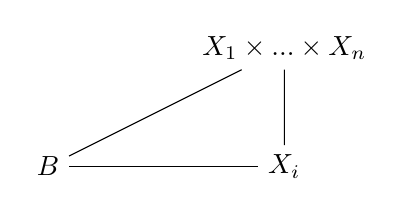
\begin{tikzpicture}[scale=1.5, auto, swap]
    \node (B) at (-1,0) {$B$};
    \node (Product) at (1,1) {$X_1\times...\times X_n$};
    \node (space) at (1,0) {$X_i$};

    \draw (B) -> (Product);
    \draw (Product) -> (space);
    \draw (B) -> (space);
  \end{tikzpicture}\\
  Just like the subspace topology, the product topology is determined by its characteristic property.\\
  \textbf{Theorem 3.11 (Uniqueness of the Product Topology):} Let $X_1,...,X_n$ be topological spaces. The product topology on $X_1\times...\times X_n$ is the unique topology that satisfies the characteristic property.\\

  We can now write the following list of properties for he product topology.\\
  \textbf{Proposition 3.12:} Let $X_1,...,X_n$ be topological spaces.

  \begin{enumerate}[label=(\alph*.)]
    \item The projection maps $\pi_i:X_1\times...\times X_n\to X_i$ are all continuous.
    \item The product topology is "associative" in the sense that the three product topologies $X_1\times X_2\times X_3$, $(X_1\times X_2) \times X_3$, and $X_1\times (X_2\times X_3)$ on the set $X_1\times X_2\times X_3$ are all equivalent.
    \item For any $i$ and any points $x_j\in X_j$, $j\neq i$, the map $f_i:X_i\to X_1\times ...\times X_n$ given by $f_i(x)=(x_1,...,x_{i-1},x,x_{i+1},...,x_n)$ is a topological embedding of $X_i$ into the product space.
    \item If for each $i$, $\mathcal{B}_i$ is a basis for the topology of $X_i$, then the set\begin{equation*}
        \{B_1\times ...\times B_n:B_i\in\mathcal{B}_i\}
    \end{equation*}
    is a basis for the product topology on $X_1\times...\times X_n$
    \item If $A_i$ is a subspace of $X$, for $i=1,...,n$, the product topology and the subspace topology on $A_1\times...\times A_n\subset X_1\times ...\times X_n$ are equal.
    \item If each $X_i$ is Hausdorff, so is $X_1\times ...\times X_n$.
    \item If each $X_i$ is second countable, so is $X_1\times ... \times X_n$.
  \end{enumerate}
  \textbf{Exercise 3.7:} Prove Proposition 3.12.

  \textbf{Proof (a.):} Let $U\subset X_i$ be an open set in $X_i$. Then it follows that $\pi_i^{-1}(U)=X_1\times ...\times X_{i-1}\times U\times X_{i+1}\times...\times X_n$. Since each set $X_k$ is open in $X_k$ and $U$ is open in $X_i$, it follows that $\pi_i^{-1}(U)$ is open in the product topology. $\square$.\\
  \\
  \textbf{Proof (b.):}\\


  \subsection{Quotient Spaces}
  Let $X$ be a topological space, $Y$ be any set, and $\pi:X\to Y$ be a surjective map. Define a topology on $Y$ by declaring a subset $U\subset Y$ to be open iff $\pi^{-1}(U)$ is open in $X$. This is called the quotient topology induced by the map $\pi$.\\
  \\
  \textbf{Exercise 3.8:} Show that the quotient topology is indeed a topology.\\
  \\
  \textbf{Proof:} Let $\mathcal{T}$ be the quotient topology on $Y$. First we need to show that $Y,\emptyset\in\mathcal{T}$. Take the inverse of $Y$, $\pi^{-1}(Y)$. This is simply the set $X$, which is obviously open in $X$. Thus, $Y\in\mathcal{T}$. Now observe $\emptyset\subset Y$. If we take the inverse image it follows that $\pi^{-1}(\emptyset)=\emptyset$ which is obviously open in $X$. Now let $Y_1,...,Y_n\in\mathcal{T}$. Then it follows that $\pi^{-1}(Y_1),...,\pi^{-1}(Y_n)$ are open in $X$. Taking the inverse image of their intersection we see: $\pi^{-1}(Y_1\cap...\cap Y_n)=\pi^{-1}(Y_1)\cap...\cap\pi^{-1}(Y_n)$. Which is just the finite intersection of open sets in $X$. Which is obviously open in $X$. Now let $A_\alpha$ be an arbitrary collection of elements of $\mathcal{T}$. We need to show that $\bigcup_\alpha A_\alpha$ also exists in $\mathcal{T}$. Take $\pi^{-1}(\bigcup_\alpha A_\alpha)=\bigcup_\alpha\pi^{-1}(A_\alpha)$. This is just an arbitrary union of open sets in $X$. Thus, it is also closed in $X$. $\square$.\\
  \\

  The most common source of quotient maps is the following construction.\\
  Let $\sim$ be an equivalence relation on a topological space $X$. For each $q\in X$ let $[q]$ denote the equivalence class of $q$, and let $X\setminus \sim$ denote the set of equivalence classes: This is a partition of $X$, which is a decomposition of $X$ into a collection of disjoint subsets whose union is $X$. let $\pi:X\to X\setminus\sim$ be the natural projection sending each element of $x$ to its equivalence class. Then $X\setminus \sim$ togeter with the quotient topology determined by $\pi$ is called the quotient space of $X$ by the given equivalence relation. The quotient map $\pi$ is called the projection. We can also define a quotient space explicitly via a partition.\\
  If $\pi:X\to Y$ is a quotient map, a subset $U\subset X$ is said to be saturated if $U=\pi^{-1}(V)$ for some subset $V\subset Y$. If $Y$ is a quotient space determined by an equivalence relation, the saturated sets are those that are unions of equivalence classes. More generally, for any quotient map $\pi:X\to Y$, a subset $\pi^{-1}(y) \subset X$ for $y\in Y$ is called a fiber of $\pi$; A saturated set is one that is a union of fibers.\\
  \textbf{Lemma 3.16:} A continuous surjective map $\pi:X\to Y$ is a quotient map iff it takes saturated open sets to open sets, or saturated closed sets to closed set.\\
  \textbf{Exercise 3.16:} Prove Lemma 3.16.\\
  \\
  \textbf{Proof:} $(\to)$ Assume $\pi:X\to Y$ is a quotient map. Now let $U\subset X$ be an open saturated set of $X$. Then it follows that $U=\pi^{-1}(\pi(U))$. Since $Y$ has the quotient topology and $\pi^{-1}(\pi(U))$ is open, it follows that $\pi(U)$ is open.\\
  \\
  $(\leftarrow)$ Now assume $\pi:X\to Y$ takes open saturated sets to open sets. Now, let $V\subset Y$ be an open set. Then it follows that $\pi^{-1}(V)$ is open by continuity.\\
  Since $\pi$ is surjective we know that $\exists Z\subset X$ such that $V=\pi(Z)$ where $\pi^{-1}(\pi(Z))=Z$. It follows that $Z$ is obviously saturated. Assume that $\pi^{-1}(V)$ is open, then it follows that $\pi^{-1}(V)=\pi^{-1}(\pi(Z))=Z$ is open. Since $Z$ is saturated and open it follows that $\pi(Z)=V$ is open. $\square$.\\
  \textbf{Lemma 3.17:} Suppose $f:X\to Y$ is a quotient map. The restriction of $f$ to any saturated open or closed set is a quotient map.\\
  \textbf{Exercise 3.10:} Prove Lemma 3.17\\
  \\
  \textbf{Proof:} Assume $f:X\to Y$ is quotient map. Let $U\subset X$ be a saturated open set. Then it follows that $\pi^{-1}(\pi(U)) = U$. \textbf{FINISH LATER}\\
  \textbf{Lemma 3.19:} If $\pi:X\to Y$ is a surjective continuous map that is also an open or closed map, then it is a quotient map.\\
  \\
  Quotient maps also behave well under composition.\\
  \textbf{Lemma 3.20:} Suppose $\pi_1:X\to Y$ and $\pi_2:Y\to Z$ are quotient maps. Then their composition $\pi_2\circ \pi_1:X\to Z$ is also a quotient map.\\
  \\
  Quotient spaces do not generally behave well with respect to products, subspaces, bases, or topological properties such as locally Euclidean, Hausdorff, or second countable. In particular the quotient spaces of manifolds are often not manifolds.\\
  If we wish to prove a given space is a manifold we have to prove at least locally Euclidean and Hausdorff properties directly.\\

  \textbf{Lemma 3.21:} Suppose $P$ is a second countable space and $\pi: P\to M$ is a quotient map. If $M$ is locally Euclidean, it is second countable.\\

  \textbf{Example 3.28:} Define \(\mathbb{P}\), the \textit{real projective space} of dimension \(n\), to be the set of \(1\)-dimensional linear subspaces (lines through the origin) in \(\mathbb{R}^{n+1}\). There is a natural map \(\pi:\mathbb{R}^{n+1}\setminus\{0\}\to \mathbb{P}^n\) defined by sending a point \(x\) to its span. We topologize \(\mathbb{P}^n\) by giving it the quotient topology with respect to this map.\\
  We can also view this space in another way. If we define an equivalence relation on \(\mathbb{R}^{n+1}\setminus\{0\}\) by declaring two points \(x,y\) to be equivalent if \(x=\lambda y\) for some nonzero real number \(\lambda\), then there is an obvious identifiction between \(\mathbb{P}^n\) and the set of equivalence classes. Under this identification, the map \(\pi\) defined above is just the map sending a point to its equivalence class.

  We know begin looking at the characteristic property of the Quotient Topology.\\
  \textbf{Theorem 3.29 (Characteristic property of quotient topologies):} Let \(\pi:X\to Y\) be a quotient map. For any topological space \(B\), a map \(f:Y\to B\) is continuous if and only if the composite map \(f\circ \pi\) is continuous.\\

  \textbf{Proof:} If \(f\) is continuous, \(f\circ\pi\) is continuous by composition. Conversely, if \(f\circ\pi\) is continuous and \(U\subset B\) is open, then \(\pi^{-1}(f^{-1}(U))=(f\circ\pi)^{-1}(U)\) is open in \(X\), which implies \(f^{-1}(U)\) is open in \(Y\) by definition of the quotient topology. Thus \(f\) is continuous. \(\square\).\\
  \\
  There is also an extremely important corollary to the characteristic property:\\
  \textbf{Corollary 3.30 (Passing to the Quotient):} Suppose \(\pi:X\to Y\) is a quotient map, \(B\) is a topological space, and \(f:X\to B\) is any continuous map that is constant on the fibers of \(\pi\) (i.e. \(\pi(p)=\pi(q)\), then \(f(p)=f(q)\). Then there exists a unique continuous map $\tilde{f}:Y\to B$ such that \(f=\tilde{f}\circ\pi\).\\
  \textbf{Proof:} The existence and uniqueness of \(\tilde{f}\) follow from elementary set theory: Given \(q\in Y\), there is some \(p\in X\) such that \(\pi(p)=q\), an we can set \(\tilde{f}(q)=f(p)\). The hypothesis on \(f\) guarantees that \(\tilde{f}\) is unique and well-defined. Continuity of \(\tilde{f}\) is then immediate from the characteristic property. \(\square\).\\

  In the situation of this previous corollary, we sy that the map \(f\) \textit{passes to the quotient} or \textit{descends to the quotient.}\\
  There are two slightly different ways of phrasing the uniqueness associated with the characteristic property.\\
  \textbf{Theorem 3.31 (Characterization of Quotient Maps):} Let \(X\) and \(Y\) be topological spaces, and let \(\pi:X\to Y\) be any surjective map. Then \(\pi\) is a quotient map iff the characteristic property holds.\\

  \textbf{Corollary 3.32 (Uniqueness of Quotient Spaces):} Suppose \(\pi_1:X\to Y_1\) and \(\pi_2:X\to Y_2\) are quotient maps that make the same identifications (i.e., \(\pi_1(p)=\pi_1(q)\) iff \(\pi_2(p)=\pi_2(q)\)). Then there is a unique homeomorphism \(\phi:Y_1\to Y_2\) such that \(\phi\circ \pi_1=\pi_2\).\\
  \subsection{Group Actions}
  \textbf{Defn:} A \textit{topological group} is a group \(G\) endowed with a topology such that the maps \(\mu:G\times G\to G\) and \(i:G\to G\) given by \[
  \mu(g_1,g_2)=g_1g_2 \text{ and } i(g)=g^{-1}
  \] are continuous, where the product and inverse are those of the group structure of \(G\).\\
  \\
  A \textit{discrete group} is a topological group that has the discrete topology.\\
  Some examples of topological groups include:
  \begin{itemize}
      \item The real line \(\mathbb{R}\) with its additive group structure and Euclidean topology.
      \item The set \(\mathbb{R}^* =\mathbb{R}\setminus \{0\}\) of nonzero real numbers under multiplication with the subspace topology.
      \item The set \(\mathbb{C}^*=\mathbb{C}\setminus\{0\}\) of nonzero complex numbers under complex multiplication, with the subspace topology.
      \item The general linear group \(GL(n,\mathbb{R})\), which is the set of \(n\times n\) invertible real matrices under matrix multiplication, with the subspace topology inherited from \(\mathbb{R}^{n^2}\).
      \item Any group with the discrete topology.
  \end{itemize}
  \textbf{Exercise 3.11:} Verify that each of the above examples is a topological group.\\
  \textbf{Proof:}
  \begin{itemize}
      \item We simply need to show that the maps \(\mu:\mathbb{R}\times\mathbb{R}\to \mathbb{R}\), \(i:\mathbb{R}\to\mathbb{R}\), where \(\mu(a,b)=a+b\) and \(i(a)=-a\) are continuous on the euclidean basis of the euclidean topology. For \(\mu\) let \(U\subset\mathbb{R}\) be an open interval of the form \((a,b)\) where \(a,b\in \mathbb{R}\). It follows that \(\mu^{-1}((a,b)) = \{(x,y):a<x+y<b\}\) which is simply a "infinite parallelogram" in the plane. Consider some point \((x,y)\in \mu^{-1}((a,b))\). We will let the sets \(\partial a=\{(x,y):x+y=a\}\) and \(\partial b=\{(x,y):x+y=b\}\) be the boundary lines of the "parallelogram". Take  \(\lambda_a=min\{d((x,y),d): d\in\partial a\}\) and \(\lambda_b=min\{d((x,y), d):d\in\partial b\}\). Then it follows that if we take $\lambda=min\{\lambda_a,\lambda_b\}$. Then it follows that the open set \((x-\lambda/2, x+\lambda/2)\times(y-\lambda/2, y+\lambda/2)\) contains \((x,y)\) and is contained in the inverse set. Thus we can take the union of all these open sets, to construct the inverse set.\\
      Phew, now we show the much easier fact that \(i\) is continuous. Let \((a,b)\) be an open interval in \(\mathbb{R}\). Then it follows that \(i^{-1}(a,b)=(-b,-a)\) which is obviously open in \(\mathbb{R}\). \(\square\).\\
      \item \textbf{COME BACK TO THIS LATER NEEDS A LOT OF WORK} We need to show that the maps \(\mu:\mathbb{R}^*\times \mathbb{R}^*\to \mathbb{R}^*\), \(i:\mathbb{R}^*\to\mathbb{R}^*\) where \(\mu(a,b)=ab\) and \(i(a)=1/a\) are continuous on the subspace topology. First we show continuity for the inverse map. Let \((a,b)\setminus\{0\}\) be an open basis element for the subspace topology. We look at the following two cases a,b has the same polarity and a,b have different polarity.\\
      Case 1: Assume \(a,b\) are both positive. Then it follows that \(i^{-1}((a,b))=(1/b,1/a)\) which is obviously open.\\
      Case 2: Assume \(a\) is negative and \(b\) is positive. Then it follows that \(i^{-1}((a,b)\setminus\{0\})=(1/a, 1/b)\setminus \{0\}\). Which is open in \(\mathbb{R}^*\).\\
      Case 3: Now assume \(a,b\) are both negative, then it follows that \(i^{-1}((a,b))=(1/b, 1/a)\), which is open in \(\mathbb{R}^*\).\\
      Now we show that \(\mu\) is continuous. Let \((a,b)\setminus\{0\}\) be a basis element for the subspace topology on \(\mathbb{R}^*\). Then it follows that \(I=\mu^{-1}((a,b)\setminus\{0\})=\{(x,y)\in\mathbb{R}^{2*}:a<xy<b\}\). Now, let $(x,y)\in I$. Thus, we have that \(a<xy<b\). We introduce the \(m(z)=\min(|z-a|, |z-b|)\) operator, to take the minimum distance between x and \(a\) and \(x\) and \(b\). Now take the point \((x-\sqrt{m(x)}/4, y-\sqrt{m(y)}/4)\)
  \end{itemize}

  \textbf{Lemma 3.34:} Any subgroup of a topological group is a topological group with the subspace topology. Any finite product of topological groups is a topological group with the direct product group structure and the product topology.\\

  \textbf{Exercise 3.34:} Prove Lemma 3.34\\
  \textbf{Proof:} Let \(G\) be a topological group with some topology \(\mathcal{T}\). \textbf{Proof Completed on Blackboard, need to transfer over}\\
  \\
  If \(G\) is a topological group and \(g\in G\), the left translation map \(L_g:G\to G\) defined by \(L_g(g')=gg'\) is continuous, because it is the restriction of the multiplication map to \(\{g\}\times G\). Because, \(L_g\circ L_g^{-1}=Id_G\), left translation by any element of \(g\) is a homeomorphism of \(G\). Similarly, right translation \(R_g(g')=g'g\) is also a homeomorphism.\\
  We now define a \textbf{left action}. Suppose \(G\) is a group and \(X\) is a topological space. A \textit{left action} of \(G\) on \(X\) is a map \(G\times X\to X\), written \((g,x)\mapsto g\cdot x\) with the following properties:
  \begin{enumerate}[label=(\Roman*.)]
      \item For any \(x\in X\) and any \(g_1,g_2\in G\), we have \(g_1\cdot (g_2\cdot x)=(g_1g_2)\cdot x\).
      \item For all \(x\in X, 1\cdot x=x\).
  \end{enumerate} 
  A \textit{right action} is is a map \(X\times G\to X\), written \((x,g)\mapsto x\cdot g\), with the same properties but composition works in reverse: \((x\cdot g_1)\cdot g_2=x\cdot (g_1g_2)\).\\
  Any right action determines a left action and vice versa via the correspondence:\[
  g\cdot x=x\cdot g^{-1}
  \]
  This means the the choice of left or right action is a matter of taste. We will usually assume/prfer to use left actions as they are often more natural.\\
  If \(G\) is a topological group, an action of \(G\) on a space \(X\) is said to be continuous if the map \(G\times X\to X\) is continuous. This means, in particular, that for each \(g\in G\) the map \(x\mapsto g\cdot x\) is continuous from \(X\) to itself, because it is the restriction of the action to the subspace \(\{g\}\times X\subset G\times X\).Each such map is a homeomorphism, because the definition of a group action guarantees it has a continuous inverse \(x\mapsto g^{-1}\cdot x\).\\
  \begin{itemize}
      \item For any \(x\in X\), the set \(G\cdot x=\{g\cdot x:g\in G\}\) is called the \textit{orbit} of \(x\).
      \item The action is said to be transitive if for every pair \(x,y\in X\) there exists \(g\in G\) such that \(g\cdot x=y\) or equivalently if the only orbit is the entire space \(X\).
      \item It is said to be free if the only element of \(G\) that has any fixed points is the identity, i.e. \(g\cdot x=x\) implies that \(g=1\).
  \end{itemize}

  Given an action \(G\) on a space \(X\), we define an equivalence relation on \(X\) by setting \(x_1\sim x_2\) if  there is an element \(g\in G\) suc that \(g\cdot x_1 = x_2\). The equivalence classes are precisely the orbits of the group action.\\
  The resulting quotient space is denoted by \(X\setminus G\), and is called the \textit{orbit space} of the action. If the action is transitive, the orbit space is a single point, so only nontransitive actions yield interesting examples.\\
  \textbf{Exercise 3.13:} Verify that the real projective space \(\mathbb{P}^n\) of example 3.28 is the orbit space of the action of \(\mathbb{R}^*\) on \(\mathbb{R}^{n+1}\setminus\{0\}\) by scalar multiplication.\\
  \\

  \textbf{Proof: } We simply need to show that the equivalence classes of lines through the origin in \(\mathbb{R}^{n+1}\setminus\{0\}\) are the same as the orbits of \(\mathbb{R}^*\) acting on \(\mathbb{R}^{n+1}\setminus\{0\}\). For each of the orbits \(O_x\) (\(x\in \mathbb{R}^{n+1}\setminus \{0\}\)) it follows that \(x'\in O_x\) iff \(g \cdot x=x'\), where \(g\in \mathbb{R}^*\). It is then obvious that \(O_x\) is simply a single all vectors in \(\mathbb{R}^{n+1}\setminus\{0\}\) that are linearly dependent with \(x\). In other words, each element of \(O_x\) sits on the same line through the origin in \(\mathbb{R}^{n+1}\setminus\{0\}\). Varying \(x\), we see that every line that passes through the origin in \(\mathbb{R}^{n+1}\setminus\{0\}\) has its own equivalence class. This is the same as the equivalence classes defined by \(\mathbb{P}^n\). Therefore, \((\mathbb{R}^{n+1}\setminus\{0\})/\mathbb{R}^*=(\mathbb{R}^{n+1}\setminus\{0\})/\mathbb{P}^n\). \(\square\).\\
  \\
  A particularly important special case arises when we consider a subgroup \(\Gamma\) of a topological group \(G\) (with subspace topology). Group multiplication on the left or right defines a left or right action of \(\Gamma\) on \(G\). it is just the restriction of the action of \(G\) on itself to \(\Gamma\times G\) or \(G\times \Gamma\). This action is continuous and free, but in general not transitive. An orbit of the right action of \(\Gamma\) on \(G\) is a set of the form \(\{g\gamma:\gamma\in\Gamma\}\), which is precisely the left coset \(g\Gamma\). Thus the orbit space of the right action of \(\Gamma\) on \(G\) is the set \(G/\Gamma \) of left cosets with the quotient topology. This quotient space is called the (left) \textit{coset space} of \(G\) on \(\Gamma\).

  \subsection{Problems:}

  \textbf{Problem 3.1:} Show that a finite product of open maps is open, and a finite product of closed maps is closed.\\
  \textbf{Proof:} Assume \(f_1:X_1\to Y_1\),...,\(f_n:X_n\to Y_n\) are open maps. Now let \(U_1\times...\times U_n\) be a basis element of \(X_1\times...\times X_n\). Then it follows that \(f(U_1\times...\times U_n)=f(U_1)\times...\times f(U_n)\). Which is a product of open sets, obviously open in \(Y_1\times ...\times Y_n\). \(\square\).\\
  \\
  \textbf{Problem 3.4:} Use stereographic projection to show that any closed ball in \(\mathbb{R}^n\) is an \(n\)-dimensional manifold with boundary.\\
  \\
  \textbf{Proof:} We know that a closed ball, \(\bar{B}(a,r)\), in \(\mathbb{R}^n\) is a  closed subspace, thus the properties of Hausdorff and Second-countability are instantly inherited from \(\mathbb{R}^n\). It then follows that We just need to show that any point in the closed ball has a neighborhood which is homeomorphic to an open subset of \(\mathbb{H}^n=\{(x_1,...,x_n)\in\mathbb{R}^n:x_n\geq 0\}\). All closed balls in \(\mathbb{R}^n\) are homeomorphic to the unit-closed ball. Thus, we will only discuss the homeomorphism from this unit-closed ball. Let \(x\in \bar{B}_1(0)\), where \(N=(1,...,1)\) and \(x\neq N\). We know that the set \(\bar{B}_1(0)\setminus \{N\}\) is open as a consequence of Hausdorffedness. Thus, take \(x\in\bar{B}_1(0)\setminus\{N\}\subset \bar{B}_1(0)\). We can extend the stereographic projection function like so, 
  \(\sigma(x_1,...,x_n):\bar{B}_1(0)\setminus \{N\}\to \mathbb{R}^{n-1}\times [0,1)\) where \(\sigma(x_1,...,x_n)=(\dfrac{x_1}{1-x_n},...,\dfrac{x_{n-1}}{1-x_n},\dfrac{x_n}{1-x_n})\).

  \textbf{Problem 3.15:} Let \(G\) be a topological group acting continuously on a topological space \(X\).
  \begin{enumerate}[label=(\alph*.)]
      \item Show that the quotient map \(\pi: X\to X/G\) is open.
      \item Show that \(X/G\) is Hausdorff iff the orbit relation \(\{(x_1,x_2\in X\times X:x_2=g\cdot x_1 \text{ for some }g\in G\}\).
  \end{enumerate}

  \textbf{Proof (a.):} Assume \(G\) is a topological group acting continuously on a topological space \(X\). Thus the map \(G\times X\to X\) is continuous. Now let \(\pi:X\to X/G\) be a quotient map. Let \(U\subset X\) be an open set in \(X\). We now define the set \(U^{-1}=\{(g,x)\in G\times X: g\cdot x\in U\}\). We know that \(U^{-1}\) is open since the map \(G\times X\to X\) is continuous. 

  \section{Connectedness and Compactness}
A space is connected iff it is not homeomorphic to a disjoint union of two or more nonempty spaces. This definition is constructed so that connected spaces will behave similarly to intervals in the real line. The definition of compactness is chosen so that compact topological spaces will have many of the same properties enjoyed by closed and bounded subsets of Euclidean spaces.
\subsection{Definitions and Basic Properties}
A topological space \(X\) is said to be \textbf{disconnected} if it can be expressed aas the union of two dijoint, nonempty, open subsets. Any suche subsets are said to disconnect \(X\).\\
If \(X\) is not disconnected, it is said to be \textbf{connected}.\\
We also provide an alternative characterization of connectedness.
\textbf{Proposition 4.1:} A topological space \(X\) is connected iff the only subsets of \(X\) that are both open and closed in \(X\) are \(\emptyset\) and \(X\) itself.\\

This characterization can often be used to prove that some subset of a connected space is equal to the whole space.\\

\textbf{Proposition 4.2:} Suppose \(X\) is a nonempty connected space. Then every continuous map from \(X\) to a discrete space is constant.\\

\textbf{Proof:} Let \(Y\) be a discrete space, and suppose \(f:X\to Y\) is continuous. Choose any \(x\in X\), and let \(c=f(x)\). The singleton \(\{c\}\) is both open and closed in \(Y\). Since, \(f\) is continuous \(f^{-1}(c)\) must also be closed and open in \(X\). Since it is not empty by hypothesis, it must be all of \(X\). Thus \(f\) is constant.\(\square\).\\

  \section{Simplicial Complexes}

  \begin{itemize}
      \item Simplical complexes are spaces constructed from building blocks called simplices, which are points, line segments, filled-in traingles, solid tetrahedra, etc..
      \item We think of a simplicial complex as a collecction of simplicies in some Euclidean space that overlap "nicely"
  \end{itemize}
  \subsection{Euclidean Simplicial Complexes}
  \begin{itemize}
      \item  An \textit{affine map} between two vector spaces is a map $f:V\to W$ of the form $f(x)=a(x)+b$, where a is a linear map and $b\in W$.
      \item An \textit{affine subspace} of a vector space is the zero set of some affine map: $\{x:a(x)+b=0\}$. Its dimension is the dimension of the kernel of the linear part of the affine map.
      \item The \textit{special case} of an affine subspace of $V$ whose dimension is one less than that of $V$ is called an affine hyperplane in $V$.
      \item if $n\geq k$, any $k+1$ points $v_0,...,v_k$ in $\mathbb{R}^n$ are contained some $k$-dimensional affine subspace.
      \item We say that $k+1$ points are in \textit{general position} if they are not contained in any $(k-1)$-dimensional affine subspace, or equivalently $\{v_1-v_0,...,v_k-v_0\}$ are linearly independent.
  \end{itemize}
  Given points $v_0,...,v_k$ in general position in $\mathbb{R}^n$, the simplex spanned by them is the set of all points in $\mathbb{R}^n$ of the form:
  \begin{equation*}
      \sum\limits_{i=0}\limits^{k}t_iv_i, \text{ where }0\leq t_i \leq 1 \text{ and }\sum\limits_{i=0}\limits^{k}t_i=1
  \end{equation*}
  with the subspace topology. Each of the points $v_i$ is called a vertex of the simplex. We will sometimes use the notation $\langle v_0,...,v_k\rangle$ to denote the simplex spanned by $v_0,...,v_k$. The integer $k$ is called the dimension of the simplex. A $k$-dimensional simplex is often called a $k$-simplex.\\
  \\
  For any subset $A\subset \mathbb{R}^n$, the convex hull of $A$ is defined to be the intersection of all convex sets containing $A$.\\
  (Refresher, any subset $B\subset \mathbb{R}^n$ is called convex if for any $x,x'\in B$ the line segment from $x$ to $x'$ lies entirely in $B$.
  
  
 \end{document}
